%; whizzy chapter
% -initex iniptex -latex platex -format platex -bibtex jbibtex -fmt fmt
% $B0J>e(B whizzytex $B$r;HMQ$9$k>l9g$N@_Dj!#(B

%     Kansai Debian Meeting resources
%     Copyright (C) 2007 Takaya Yamashita
%     Thank you for Tokyo Debian Meeting resources

%     This program is free software; you can redistribute it and/or modify
%     it under the terms of the GNU General Public License as published by
%     the Free Software Foundation; either version 2 of the License, or
%     (at your option) any later version.

%     This program is distributed in the hope that it will be useful,
%     but WITHOUT ANY WARRANTY; without even the implied warranty of
%     MERCHANTABILITY or FITNESS FOR A PARTICULAR PURPOSE.  See the
%     GNU General Public License for more details.

%     You should have received a copy of the GNU General Public License
%     along with this program; if not, write to the Free Software
%     Foundation, Inc., 51 Franklin St, Fifth Floor, Boston, MA  02110-1301 USA

%  preview (shell-command (concat "evince " (replace-regexp-in-string "tex$" "pdf"(buffer-file-name)) "&"))
% $B2hA|%U%!%$%k$r=hM}$9$k$?$a$K$O(Bebb$B$rMxMQ$7$F(Bboundingbox$B$r:n@.!#(B
%(shell-command "cd image200708; ebb *.png")

%%$B$3$3$+$i%X%C%@3+;O!#(B

\documentclass[mingoth,a4paper]{jsarticle}
\usepackage{kansaimonthlyreport}
\usepackage[dvips]{xy}
\usepackage{ulem}

% $BF|IU$rDj5A$9$k!"Kh7nJQ$o$j$^$9!#(B
\newcommand{\debmtgyear}{2019}
\newcommand{\debmtgdate}{24}
\newcommand{\debmtgmonth}{3}
\newcommand{\debmtgnumber}{144}

\def\fixme#1{{\color{red}{#1}}}

\begin{document}

\begin{titlepage}

% $BKh7nJQ99$9$kItJ,!"K\J8$NKvHx$b=$@5$9$k$3$H$r$o$9$l$:$K(B

 $BBh(B\debmtgnumber{}$B2s(B $B4X@>(B Debian $BJY6/2q;qNA(B

\vspace{2cm}

\begin{center}
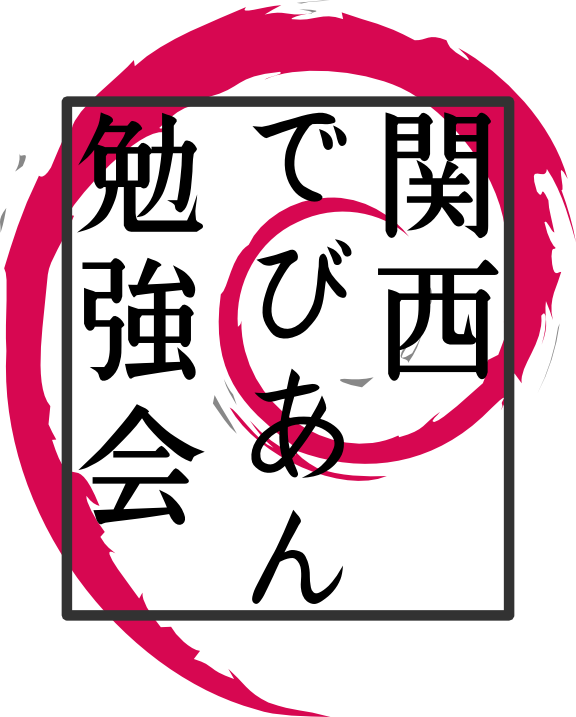
\includegraphics{image200802/kansaidebianlogo.png}
\end{center}

\begin{flushright}
\hfill{}$B4X@>(B Debian $BJY6/2qC4Ev<T(B $B:4!9LZ!&ARI_!&$N$,$?!&$+$o$@!&$*$*$D$-(B \\
\hfill{}\debmtgyear{}$BG/(B\debmtgmonth{}$B7n(B\debmtgdate{}$BF|(B
\end{flushright}

\thispagestyle{empty}
\end{titlepage}

\dancersection{$B:G6a$N(BDebian$B4X78$N%$%Y%s%HJs9p(B}{Debian JP}

\dancersection{$B;vA02]Bj(B}{$B4X@>(BDebian$BJY6/2q(B}

$B;22C<T$N3'$5$s$O0J2<$NDL$j$G$9(B:
\begin{prework}{Katsuki Kobayashi}
\end{prework}

\dancersection{\mbox{Rust$B$G=q$$$?%D!<%k$N(B}\mbox{debian$B%Q%C%1!<%8%s%0$K(B}\mbox{$BD)@o$7$F$_$?OC(B($B2>(B)}}{$B>.NS(B $B9n4u(B}

\subsection{$B$O$8$a$K(B}

$B:#2s$NFbMF$G$9$,!":G6a8D?ME*$K?($j$@$7$?(BRust$B$H$$$&%W%m%0%i%_%s%08@8l$K$D$$$F!"(B
$B$=$b$=$b$I$&$$$&8@8l$J$s$@$H$$$&$4>R2p(B($B$H$$$C$F$b!";d$bJY6/Cf$N?H$G$9$,(B)$B$H!"(B
Rust$B$G=q$$$?%D!<%k$N(Bdeb$B$r:n$C$F$_$k!"$H$$$&$H$3$m$^$G$rL\I8$H$7$F$$$^$9!#(B

\subsection{Rust$B$H$O(B}

Rust$B$H$O!"(BMozilla$B$,%V%i%&%6%(%s%8%s(BServo$B$N$?$a$K3+H/$7$?%7%9%F%`%W%m%0%i%_%s%08@8l$G$9!#(B
2018$BG/$N%9%?%C%/%*!<%P!<%U%m!<$ND4::(B%
\footnote{\url{https://insights.stackoverflow.com/survey/2018}}%
$B$G0&$5$l$F$$$k8@8l%i%s%-%s%0(B1$B0L$K$J$k$J$I!"(B
$B:G6a$G$O7k9=%a%8%c!<$K$J$C$F$$$F$$$k46$8$N8@8l$G$9!#(B
$BFCD'$H$7$F$O!"0BA4@-!&JB9T@-$K$D$$$F9M$($i$l$F@_7W$5$l$F$$$kE@$G!"(B
$B$+$D!"$_$s$JBg9%$-(B(?)$B@EE*7?IU$18@8l$G$9!#(B

$B$J$*!"(BRust$B%W%m%0%i%^!<$N;v$r(Brustacean($B%i%9%H%7%"%s(B)$B$H$$$&$h$&$G$9!#(B
$B$3$l$O!"(B``Crustacean($B9C3LN`(B)`` $B$+$iMh$F$$$k$i$7$/!"(B
$B$=$N$;$$$+!"%*%i%$%j!<K\$NI=;f$O%*%*%R%m%P%*%&%.%,%K$H$$$&%+%K$G$9$7!"(B
$BHs8x<0%^%9%3%C%H$b$+$o$$$i$7$$%+%K(B($BL>A0$O(BFerris%
\footnote{\url{http://rustacean.net/}}%
)$B$K$J$C$F$^$9!#(B

\subsubsection{Rust$B$N%D!<%k%A%'!<%s$r%$%s%9%H!<%k(B}

$B$G$O$5$C$=$/(BRust$B$N%D!<%k%A%'!<%s$r%$%s%9%H!<%k$7$F$_$^$7$g$&!#(B
$B$5$F!"$b$A$m$s(BRust$B$N%D!<%k%A%'!<%s$N(Bdebian$B%Q%C%1!<%8$O$"$j$^$9$7!"(B
$B%m!<%+%k%^%7%s$K%$%s%9%H!<%k$;$:$K%V%i%&%6$G?'!9;n$;$k%5%$%H(B%
\footnote{\url{https://play.rust-lang.org/}}
$B$b$"$k$N$G$9$,!"(BRust$B$O(B2018$BG/$NG/Kv$K(B2018 Edition%
\footnote{\url{https://blog.rust-lang.org/2018/12/06/Rust-1.31-and-rust-2018.html}}%
$B$H$$$&Bg$-$a$J2~HG$,$"$C$?$N$G!"(B
$B$R$H$^$:(BRust$B8x<0$N<jCJ$G%D!<%k%A%'!<%s$r%$%s%9%H!<%k$7$^$7$g$&!#(B
$BNc$K$h$C$FNc$N$4$H$/!"3'MM$NBg;v$J%[!<%`%G%#%l%/%H%j$K?'!9$HF~$l$F$7$^$$$^$9$,!"(B
$B%P!<%8%g%s%"%C%W$NIQEY$O$=$l$J$j$K$"$k$N$G!"(BRust$B$N:G?7$rDI$C$F$$$/$J$i!"(B
$BL5M}$;$:$K8x<0$N%D!<%k%A%'!<%s$rF~$l$F$7$^$C$?J}$,L5Fq$+$H;W$$$^$9!#(B

Rust$B$N%D!<%k%A%'!<%s$G$9$,!"0JA0$O$=$&$G$b$J$+$C$?$_$?$$$G$9$,!":G6a$G$O(Brustup%
\footnote{\url{https://rustup.rs/}}%
$B$H$$$&%$%s%9%H!<%i!<$r;H$&$N$,8x<0<j=g$N$h$&$G$9!#(B
$B$$$+$K$b:G6a$N%D!<%k$C$]$$$G$9$,!"0J2<$N$h$&$K(Bcurl$B%3%^%s%I$rC!$$$F%$%s%9%H!<%k$7$^$9!#(B

\begin{commandline}
% curl https://sh.rustup.rs -sSf | sh
\end{commandline}

rustup$B$r;H$&$H!"%P%$%J%j$O(B \verb|~/.cargo| $B0J2<$K%$%s%9%H!<%k$5$l$^$9!#(B
$B%Q%9$rDL$7$?$$>l9g!"(B \verb|~/.cargo/env| $B$H$$$&%U%!%$%k$,$"$k$N$G!"(B
$B$=$A$i$r(B \texttt{source} $B$7$F$"$2$k$H$h$m$7$$$+$H;W$$$^$9!#(B
$B$R$H$^$:!"(B \texttt{cargo} $B$H$$$&%3%^%s%I$,;H$($k$h$&$K$J$C$F$$$?$iBg>fIW$G$9!#(B
$B$J$*!"!V$I$&$7$F$b(Bdeb$B$G!W$H$$$&J}$O(B \texttt{cargo} $B%Q%C%1!<%8$r%$%s%9%H!<%k$7$F$/$@$5$$!#(B
$B$=$N:]!"(B\texttt{rustc}$B$N%P!<%8%g%s$,(B2018 Edition$B$G$"$k(B1.31$B0J9_$G$"$k;v$,K>$^$7$$$G$9!#(B

\subsubsection{Hello World$B$7$F$_$k(B}

$B$G$O!"(Bcargo$B$,;H$($k$h$&$K$J$C$?$H$3$m$G!"(BHello World$B$7$F$_$^$7$g$&!#(B
Rust$B$N%W%m%8%'%/%H$O!"(B \verb|cargo new| $B$G:n@.$9$k$3$H$,$G$-$^$9!#(B
$B@N$O(B\verb|--bin|$B$r$D$1$J$$$H%i%$%V%i%jMQ$N%W%m%8%'%/%H$K$J$C$F$^$7$?$,!"(B
$B:G6a$N(Bcargo$B$G$"$l$P%G%U%)%k%H$,%P%$%J%jMQ$N%W%m%8%'%/%H$K$J$j$^$9!#(B
$B$=$l$G$O<B9T$7$F$_$^$7$g$&!#(B

\begin{commandline}
% cargo new hello
     Created binary (application) `hello` package
% tree
.
$B('(!(!(B Cargo.toml
$B(&(!(!(B src
    $B(&(!(!(B main.rs

1 directory, 2 files
\end{commandline}

$B<B9T$9$k$H!"$3$s$J46$8$K(BCargo.toml$B$H$$$&%U%!%$%k$H!"(B
main.rs$B$H$$$&%=!<%9%U%!%$%k$,:n@.$5$l$^$9!#(B
$B$=$&!"(BRust$B$N%=!<%9%U%!%$%k$N3HD%;R$O(B.rs$B$G$9!#(B
$B$=$N$?$a!"(BRust$B$N%W%m%8%'%/%H$N%&%'%V%5%$%H$O!"(B.rs$B%I%a%$%s$G:n$i$l$F$k;v$,$*$*$$$G$9!#(B
$B$A$J$_$K!"(B.rs$B$O%;%k%S%"$N%I%a%$%s$G$9!#(B

$B<B$O!"$3$N;~E@$G(BHello World$B$NH>J,$,40N;$7$F$$$^$9!#(B
src/main.rs$B$NCf?H$r8+$F$_$^$7$g$&!#(B

\begin{commandline}
fn main() {
    println!("Hello, world!");
}
\end{commandline}

$B$J$s$H!"4{$K(BHello World$B$N%3!<%I$,@8@.$5$l$F$$$^$9!#(B
$B$J$*!">\:Y$O>J$-$^$9$,!"(B \verb|println!()| $B$O4X?t$K8+$($^$9$,!"(B
$B%S%C%/%j%^!<%/$,IU$$$F$$$kJ*$O!"(BRust$B$G$O%^%/%m$G$"$C$?$j$7$^$9!#(B
$B$^$!!"?<$/IU$-2q$&A0$O!"FC$K5$$K$7$J$/$FNI$$$+$H;W$$$^$9!#(B
$B%S%k%I$7$F<B9T$9$k$K$O(B \verb|cargo run| $B$9$l$P(BOK$B$G$9!#(B

\begin{commandline}
% cargo run
   Compiling hello v0.1.0 (/path/to/hello)
    Finished dev [unoptimized + debuginfo] target(s) in 0.31s
     Running `target/debug/hello`
Hello, world!
\end{commandline}

\subsection{Rust$B$N9=J8Ey$N>R2p(B}

$B$=$l$G$O!"$3$3$+$i$O4JC1$K(BRust$B$N9=J8Ey$N>R2p$r$7$F$$$-$?$$$H;W$$$^$9!#(B
$B$J$*!";d$bJY6/Cf$N?H$G$9$N$G!"HyL/$K13$r=q$$$F$$$?$i$9$$$^$;$s!#(B
$B@53N$J;v$O!"(BThe Book%
\footnote{\url{https://doc.rust-lang.org/book/}}%
$B$H8F$P$l$k5$9g$NF~$C$?%I%-%e%a%s%H$,$"$j$^$9$N$G$=$A$i$r;29M$K$7$F$$$?$@$1$?$i$H;W$$$^$9!#(B

$B$J$*!"(BRust$B$OHf3SE*3X=,$,Fq$7$$$H$+8@$o$l$F$^$9$,!"(B
$B$J$s$GFq$7$$$N$+$K$D$$$F!"8D?ME*$K$O%*%i%$%j!<$N(BRust$BK\$G0zMQ$5$l$F$k(BQuora$B$K=q$+$l$?%3%a%s%H(B%
\footnote{\url{https://www.quora.com/What-do-C-C++-systems-programmers-think-of-Rust/answer/Mitchell-Nordine}}%
$B$,$7$C$/$jMh$?$N$G0zMQ$7$F$*$-$^$9!#(B
\begin{quotation}
I've found that Rust has forced me to learn many of the things that I was slowly learning as
``good practise'' in C/C++ before I could even compile my code.
\end{quotation}
$B;d$O:G6a2q<R$N;E;v$N4X78$G(BC++$B$NJY6/$b$9$k%O%a$K$J$C$F$k$N$G$9$,!"$^$5$K>e5-$HF1$846A[$G$9!#(B
$B$J$K$+!"(BC++$B$,$3$J$l$FMh$F!"(BC++11$B$"$?$j$G$h$&$d$/NI$$46$8$K$J$C$?5!G=$@$1$r<h$jF~$l$F$$$C$?$N$,(B
Rust$B$J$s$8$c$J$$$+$J$!$H!#(B

\subsubsection{$BJQ?t@k8@(B}

$BJQ?t$N@k8@$O(B\texttt{let}$B%-!<%o!<%I$r;H$$$^$9!#(B
$B7?$O!":G6a$N8@8l$C$]$/%3%m%s$N8e$K=q$-$^$9$,!"7?$,?dO@$G$-$k$J$i>JN,2DG=$G$9!#(B
$B$^$?!"%7%c%I!<%$%s%0$9$k$3$H$b2DG=$G!";XDj$,$J$1$l$P(Bimmutable$B$JJQ?t$K$J$k$N$G!"(B
mutable$B$JJQ?t$r:n$k>l9g$O(B\texttt{mut}$B%-!<%o!<%I$r;H$$$^$9!#(B
$B6qBNE*$JNc$r0J2<$K<($7$^$9!#(B

\begin{commandline}
fn main() {
    let x = 1;
    println!("x = {}", x);
    let x = 1.25;
    println!("x = {}", x);
    x = 1;   // $B%(%i!<$K$J$k(B($B$=$b$=$b(Bimmutable$B$@$1$I(B): expected floating-point number, found integer
    x = 1.5; // $B%(%i!<$K$J$k(B: cannot assign twice to immutable variable

    let mut y: u32 = 1;
    y -= 1;
    y -= 1;
    println!("y = {}", y);
}
\end{commandline}

$BNc$N(B2$B$DL\$N(B\verb|y -= 1;|$B$G$9$,!"%G%P%C%0%S%k%I$@$H%*!<%P!<%U%m!<$r8!CN$7$F<B9T;~$K%Q%K%C%/$r5/$3$7$^$9!#(B
$B%j%j!<%9%S%k%I(B(\verb|--release|$B%*%W%7%g%sIU$-$G(B\texttt{cargo}$B$r<B9T(B)$B$@$H(B
$B%Q%K%C%/$OH/@8$7$^$;$s$,!"$b$A$m$s$*$+$7$JCM$,I=<($5$l$^$9!#(B

$B$J$*!"4pK\E*$J7?$O0J2<$N$h$&$J$b$N$,$"$j$^$9!#(B

\begin{quote}
\begin{description}
 \item[$B@0?t(B]
	    \textbf{$BId9fL5$7(B:} \texttt{u8}, \texttt{u16}, \texttt{u32}, \texttt{u64}, \texttt{usize}\\
	    \textbf{$BId9fIU$-(B:} \texttt{i8}, \texttt{i16}, \texttt{i32}, \texttt{i64}, \texttt{isize}
 \item[$BIbF0>.?tE@(B] \textbf{$BC1@:EY(B:} \texttt{f32}$B!"(B\textbf{$BG\@:EY(B:} \texttt{f64}
 \item[$B%V!<%k(B] \texttt{bool}
 \item[$BJ8;z(B] \texttt{char}  (Unicode$B$N(B1$BJ8;z(B)
 \item[$BJ8;zNs(B] \texttt{String}
	    \begin{itemize}
	     \item $B$?$@$7!"J8;zNs%j%F%i%k$N(B \texttt{str} $B$,$"$C$F$H$F$b$d$d$3$7$$(B
	    \end{itemize}
 \item[$BG[Ns(B] \texttt{[T; N]} (\texttt{T}: $B7?(B,  \texttt{N}: $BMWAG?t(B)
 \item[$B%Y%/%?!<(B] \texttt{Vec<T>} (\texttt{T}: $B7?(B)
 \item[$B%9%i%$%9(B] \texttt{\&[T]} (\texttt{T}: $B7?(B)
\end{description}
\end{quote}

\texttt{String}$B$H(B\texttt{str}$B$,>/!9$d$d$3$7$$$G$9$,!"(B
$B%$%a!<%8$H$7$F$O(BC++$B$N(B\texttt{std::string}$B$H(B\texttt{char}$B$N4X78$K6a$$$h$&$J46$8$G$9!#(B
\texttt{String}$B$NJ}$O2DJQD9$G!"%a%b%j>e$N%$%a!<%8$r?^$K$9$k$H?^(B\ref{fig:str-string}$B$N$h$&$J46$8$G$9!#(B
\texttt{\&}$B$,$D$$$F$k(B\texttt{str}$B$O!"$3$N8e=R$9$k;2>H$K$J$C$F$^$9!#(B
$B$R$H$^$:!"0J2<$,$A$g$C$H$7$?%5%s%W%k%3!<%I$G$9!#(B

\begin{figure}[htbp]
 \begin{center}
  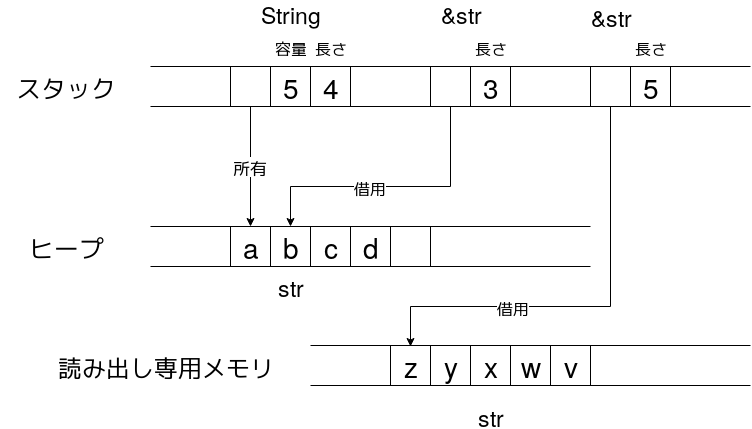
\includegraphics[keepaspectratio,height=4cm]{./image201903/rustlang-str-string.png}
  \label{fig:str-string}
  \caption{Rust$B$K$*$1$k(BString$B$H(Bstr$B$N0c$$(B}
 \end{center}
\end{figure}

\begin{commandline}
fn main() {
    let a = "abcd".to_string(); // String::from("abcd"); $B$G$b2D(B
    let b = &a[1..];
    let c = "zyxwv";

    let mut a = "abcd".to_string();
    //  ^^^  a$B$r(Bmutable$B$JJQ?t$H$7$F@k8@(B
    a.push_str("efg");  // OK

    let mut c = "zyxwv";

    // $B%(%i!<(B!: no method named `push_str` found for type `&str` in the current scope
    c.push_str("ut");  // str$B$K$ODI2C$G$-$J$$$N$G(Bpush_str$B%a%=%C%I$O$J$$(B
}
\end{commandline}

\subsubsection{$B4X?tDj5A(B}

$B$G$O!"4X?t$rDj5A$7$F$_$^$7$g$&!#(B
Rust$B$G$N4X?tDj5A$O!"(B\texttt{fn}$B%-!<%o!<%I$H(B`\texttt{->}'$B%H!<%/%s$r;H$$$^$9!#(B
$B$^$:$O!"C1=c$KB-$7;;$r9T$&4X?t(B\texttt{add}$B$rDj5A$7$F$_$^$9!#(B

\begin{commandline}
fn add(a: i32, b: i32) -> i32 {
    return a + b;
}

fn main() {
    println!("{}", add(1, 2));
}
\end{commandline}

$B$3$l$r(B\texttt{cargo}$B$G<B9T$9$k$H!"(B
($B6C$/$h$&$J;v$O0l@Z$J$$$G$9$,(B)$B0J2<$N$h$&$J7k2L$K$J$j$^$9!#(B

\begin{commandline}
% cargo run
Compiling function v0.1.0 (/path/to/examples/function)
Finished dev [unoptimized + debuginfo] target(s) in 0.20s
Running `target/debug/function`
3
\end{commandline}

$B$J$*!"$3$3$G$O(B\texttt{return}$B$r;H$$$^$7$?$,!"(B
Rust$B$G$O%;%_%3%m%s$rH4$+$9$HCM$r:n$k$?$a!"(B
$B%;%_%3%m%s$rH4$+$7$F=q$$$?0J2<$N$h$&$J(B\texttt{add}$B4X?t$b(B
$B>e5-$GDj5A$7$?4X?t$HF1$8F0:n$r$7$^$9(B($B%;%_%3%m%s$r=q$/$H%(%i!<$K$J$j$^$9(B)$B!#(B

\begin{commandline}
fn add(a: i32, b: i32) -> i32 {
    a + b
}
\end{commandline}

\subsubsection{$B=jM-8"(B}

$B$5$F!"$3$3$+$i0l5$$K(BRust$B$C$]$$OC$K$J$j$^$9!#(B
Rust$B$G$O!"%a%b%j$N0BA4@-$,9M$($i$l$F$$$k$H=q$-$^$7$?$,!"(B
$B$=$N$?$a$K=jM-8"(B($B1Q8l$G$O(Bownership)$B$H$$$&35G0$r;H$C$F$$$^$9!#(B
C++$B$G$b$"$k35G0$G$9$,!"$?$H$($P0J2<$N$h$&$J%W%m%0%i%`$,$"$C$?$H$7$^$9!#(B

\begin{commandline}
fn main() {
    let i0 = 1;
    let i1 = i0;
    let i2 = i0;

    let s0: String = "hoge".to_string();
    let s1 = s0;
    let s2 = s0;
}
\end{commandline}

$B$5$F!"$I$&$J$k$H;W$&$G$7$g$&$+(B?
$B@52r$O!"0J2<$N$h$&$K(B\texttt{s2}$B$K(B\texttt{s0}$B$rBeF~$7$F$$$k$H$3$m$G%(%i!<$K$J$j$^$9!#(B

\begin{commandline}
error[E0382]: use of moved value: `s0`
 --> ownership/src/main.rs:8:15
  |
6 |     let s0: String = "hoge".to_string();
  |         -- move occurs because `s0` has type `std::string::String`, which does not implement the `Copy` trait
7 |     let s1 = s0;
  |              -- value moved here
8 |     let s2 = s0;
  |              ^^ value used here after move
\end{commandline}

Rust$B$G$O!"BeF~!"4X?t$N0z?t!"4X?t$NLa$jCM$J$I$GCM$N=jM-8"$,0\F0$9$k$?$a!"(B
$B0lEY=jM-8"$r0\>y$7$F$7$^$C$?$i!"0\>y85$NJQ?t$O$=$N8e%"%/%;%9$G$-$J$/$J$j$^$9(B($B%3%s%Q%$%k;~$KE\$i$l$k(B)$B!#(B
$B$H$3$m$,!">e5-$N%3!<%I$G$O@0?t$NJ}$O%(%i!<$K$J$j$^$;$s!#(B
$B$3$l$O2?8N$+$H$$$&$H!"@0?t$J$I0lIt$N7?(B($B%5%$%:$,8GDj$G>.$5$$$b$N$,<g(B?)$B$O0\F0$;$:$K%3%T!<$K$J$j$^$9!#(B
$B<B$O%(%i!<%a%C%;!<%8$K$"$k(BCopy trait$B$H$$$&$N$,%_%=$G!"(B
$B@0?t7?$O$3$N(BCopy trait$B$r<BAu$7$F$$$k$+$i$=$&$$$C$?F0:n$K$J$C$F$$$^$9!#(B
trait$B$K$D$$$F$O8e=R$7$^$9!#(B

$B4X?t$N0z?t$G$b=jM-8"$O0\F0$9$k$N$G!"0J2<$N$h$&$J%3!<%I$b%"%&%H$G$9!#(B

\begin{commandline}
fn consume(_s: String) {}

fn main() {
    let h: String = "Hello World".to_string();
    consume(h);
    let hh = h;
}
\end{commandline}

$B%S%k%I$9$k$H!"4X?t(B\texttt{consume}$B%3!<%k;~$K(B\texttt{h}$B$,0\F0$7$F$7$^$C$F$$$k$?$a(B
$B0J2<$N$h$&$J%(%i!<$K$J$j$^$9!#(B

\begin{commandline}
12 |     let h: String = "Hello World".to_string();
   |         - move occurs because `h` has type `std::string::String`, which does not implement the `Copy` trait
13 |     consume(h);
   |             - value moved here
14 |     let hh = h;
   |              ^ value used here after move
\end{commandline}

$B5U$K!"4X?t$NLa$jCM$G$b=jM-8"$r0\F0$G$-$k$N$G!"0J2<$N$h$&$J%3!<%I$,=q$1$?$j$7$^$9!#(B

\begin{commandline}
fn generate(i: i32) -> Vec<i32> {
    let mut v = Vec::new();
    v.push(i);
    return v;
}

fn main() {
    let v1 = generate(10);
    let mut v2 = generate(100);
    v2.push(101);
    println!("v1: {:?}", v1); // v1: [10]
    println!("v2: {:?}", v2); // v2: [100, 101]
}
\end{commandline}

\subsubsection{$B;2>H$H<ZMQ(B}

$B4X?t8F$S=P$7$J$I$G$O!"=jM-8"$rEO$5$:$KCM$r;H$$$?$$>l9g$,B?!9$"$k$+$H;W$$$^$9$,!"(B
$B$=$N>l9g$K$O;2>H$r;H$$$^$9!#(B
$B$J$*!"(BRust$B$G$O<ZMQ$H$b8@$$$^$9!#(B
$B5-K!$H$7$F$O!"(BC++$B$HF1$8$/(B\texttt{\&}$B$r;H$&$N$G$9$,!"(B
C++$B$H$O!"(B
\begin{itemize}
 \item $B<ZMQ$9$kB&(B($B;2>H$5$l$kB&(B)$B$K(B`\texttt{\&}'$B$rIU$1$k(B
 \item $B4X?t$N8F$S=P$785$H8F$S=P$7@hN>J}$K(B`\texttt{\&}'$B$,I,MW(B
\end{itemize}
$B$H$$$C$?E@$G0[$J$k46$8$K$J$j$^$9!#(B
$B@hDx!"=jM-8"$N0\F0$G%(%i!<$K$J$C$?4X?t8F$S=P$7$N%3!<%I$r(B
$B;2>H$r$D$+$C$F%(%i!<$K$J$i$J$$$h$&$K=q$-49$($?$b$N$,0J2<$K$J$j$^$9!#(B

\begin{commandline}
fn consume(_s: &String) {}

fn main() {
    let s0: String = "hoge".to_string();
    let s1 = &s0;
    let s2 = &s0;

    let h: String = "Hello World".to_string();
    consume(&h);
    let hh = h;
}
\end{commandline}

$B$3$N%3!<%I$G$"$l$P!"4X?t(B\texttt{consume}$B$r%3!<%k$7$F$b!"(B
\texttt{h}$B$N=jM-8"$O$&$D$C$F$$$J$$$?$a!"$=$N8e(B\texttt{hh}$B$K=jM-8"$r0\>y$9$k$3$H$,$G$-$^$9!#(B
$B;2>H$N2r7h$K$O!"0J2<$N$h$&$K(B\texttt{*}$B$r;H$$$^$9!#(B

\begin{commandline}
fn main() {
    let i0 = 5;
    let i1 = &i0;

    println!("i0: {}, i1: {}", i0, *i1);
}
\end{commandline}

$B$,!"4X?t$G;H$&>l9g$@$C$?$j!"?'!9$J>lLL$G>JN,$G$-$?$j$9$k$_$?$$$G$9!#(B

\begin{commandline}
fn catlength(a: &String, b: &String) -> usize {
    return a.len() + b.len();
}

fn main() {
    let s0 = "hoge".to_string();
    let s1 = "fuga".to_string();
    println!("{}", catlength(&s0, &s1));
}
\end{commandline}

\subsubsection{$B%i%$%U%?%$%`(B}

Rust$B$K$O!"(BGC$B$O$J$/$F(BC$B8@8l$N$h$&$KJQ?t%9%3!<%W$,$"$j!"(B
$B%9%3!<%W$r30$l$?JQ?t$O?o;~>C$($F$$$-$^$9!#(B
$BNc$H$7$F$O!"0J2<$N$h$&$J%3!<%I$r=q$/$H!"(B
$B%I%m%C%W$5$l$?8e$KCM$r;H$*$&$H$7$F$$$k$?$a%3%s%Q%$%k;~$NE\$i$l$^$9!#(B

\begin{commandline}
fn main() {
    {
        let a = 0;
    }  // $B$3$3$G%I%m%C%W(B
    println!("{}", a);
}
\end{commandline}

$B<B9T$9$k$H0J2<$N$h$&$KE\$i$l$^$9!#(B

\begin{commandline}
error[E0425]: cannot find value `a` in this scope
--> lifetime/src/main.rs:5:20
  |
5 |     println!("{}", a);
  |                    ^ not found in this scope
\end{commandline}

$B;2>H$7$F$$$k>l9g$H$FE\$i$l$^$9!#(B
$BNc$H$7$F!"0J2<$N$h$&$J%3!<%I$r=q$-$^$9!#(B

\begin{commandline}
fn main() {
    let r;
    {
        let b = 0;
        r = &b;
    }
    println!("{}", r);
}
\end{commandline}

$B%3%s%Q%$%k;~$KE\$i$l$^$9!#(B

\begin{commandline}
error[E0597]: `b` does not live long enough
--> lifetime/src/main.rs:11:9
   |
11 |         r = &b;
   |         ^^^^^^ borrowed value does not live long enough
12 |     }
   |     - `b` dropped here while still borrowed
13 |     println!("{}", r);
   |                    - borrow later used here
\end{commandline}

$B$G$b!"<B$O$3$N(B\textbf{$B!V%3%s%Q%$%k;~$NE\$i$l$k!W(B}$B$H$$$&$N$,%_%=$J$N$G$9!#(B
C/C++$B$G$h$/$d$k2rJ|:Q$_$N%a%b%j%"%/%;%9$H$+$,(B
$B%3%s%Q%$%k;~$K$_$D$+$k$N$G$9!#AGE((B!!
$B$H$O$$$(!"$d$d$3$7$$$N$,4X?t$G$9!#0J2<$,%(%i!<$K$J$j$^$9!#(B

\begin{commandline}
fn longest(x: &str, y: &str) -> &str {
    if x.len() > y.len() {
        x
    } else {
        y
    }
}
\end{commandline}

$B$3$s$J46$8$GE\$i$l$^$9!#(B

\begin{commandline}
error[E0106]: missing lifetime specifier
--> lifetime/src/main.rs:1:33
  |
1 | fn longest(x: &str, y: &str) -> &str {
  |                                 ^ expected lifetime parameter
  |
= help: this function's return type contains a borrowed value, but the signature does not say whether it is \
borrowed from `x` or `y`
\end{commandline}

$B$3$N%3!<%I$NLdBj$O$J$K$+$H$$$&$H!"(B
$B<B9T$9$k$^$G(B\texttt{x}$B$H(B\texttt{y}($B$I$A$i$b;2>H(B)$B$N$I$A$i$rJV$9$+$o$+$i$J$$$N$G!"(B
$BLa$jCM$N%i%$%U%?%$%`$,$I$&$J$k$+$o$+$i$J$$$N$G!"(B
$B$=$N8e$N=hM}$,%A%'%C%/$G$-$J$$$H$$$&;v$GE\$i$l$F$$$^$9!#(B
$B$G$O$I$&$9$k$+$H$$$&$H!"%3%s%Q%$%i$,8@$C$F$$$kDL$j(Blifetime parameter$B$rDI2C$7$^$9!#(B
$B6qBNE*$K$O!"@8B84|4V(B\texttt{'a}$B$H$$$&I=8=$rMQ$$$F0J2<$N$h$&$K=q$-$^$9!#(B

\begin{commandline}
fn longest<'a>(x: &'a str, y: &'a str) -> &'a str {
    if x.len() > y.len() {
        x
    } else {
        y
    }
}
\end{commandline}

$B$3$l$K$h$C$F!"$3$N4X?t(B\texttt{longest}$B$NLa$jCM$O!"(B
\texttt{x}$B$+(B\texttt{y}$B$NC;$$J}$N%i%$%U%?%$%`0J>e$N%i%$%U%?%$%`$r;}$D$H$$$&5-:\$K$J$j!"(B
$B%3%s%Q%$%i$O$3$l$K$h$C$FCM$N<ZMQ$N%A%'%C%/$r9T$J$$$^$9!#(B

\subsubsection{$B9=B$BN(B}

Rust$B$K$O(Bclass$B$,$J$/!"9=B$BN(B\texttt{struct}$B$r;H$$$^$9!#(B
$BDj5A$O(BC$B8@8l$N9=B$BN$HF1$8$h$&$J(B($B7?$O8eCV$K$J$j$^$9(B)$B46$8$G$9$,!"(B
$B@k8@$9$k>l9g$O3FMWAG$NL>A0$rC`0l=q$/I,MW$,$"$j$^$9!#(B
$B$?$@$7!"MWAGL>$HF1L>$NJQ?t$G=i4|2=$9$k$H$-$N$_>JN,2DG=$G$9!#(B
$B$"$H$O!"B>$NJQ?t$+$iCM$r%3%T!<$7$F0lIt$@$1CM$rF~$l$k$H$$$C$?5-K!$b$"$j$^$9!#(B

\begin{commandline}
struct Point {
    x: f64,
    y: f64,
}

fn main() {
    let _p0 = Point { x: 1.0, y: 1.0 };

    let x = 0.0;
    let y = 0.0;
    let _p1 = Point { x, y }; // $BJQ?tL>$H%a%s%P!<L>$,0l=o(B
}
\end{commandline}

$B$J$*!"9=B$BN$G$9$,!"%a%=%C%I$r@8$d$9$3$H$,$G$-$^$9!#(B
$B$=$N:]!"(B\texttt{impl}$B%-!<%o!<%I$rMQ$$$F!"9=B$BN$NDj5A$+$iN%$l$?>l=j$K=q$-$^$9!#(B
$B3F4X?t$N:G=i$N0z?t$OFCJL$J0z?t$G$"$k(B\texttt{self}$B$X$N;2>H$G$"$kI,MW$,$"$j$^$9!#(B
$B%a%s%P!<$NCM$r=q$-49$($?$$>l9g$O(B\texttt{mut}$B$rIU$1$^$9!#(B

\begin{commandline}
struct Point {
    x: f64,
    y: f64,
}

impl Point {
    fn abs(&self) -> f64 {
        (self.x * self.x + self.y * self.y).sqrt()
    }
}

fn main() {
    let p0 = Point { x: 1.0, y: 1.0 };
    println!("{}", p0.abs()); // => 1.4142135623730951
}
\end{commandline}

\subsubsection{$B%8%'%M%j%C%/(B}

C++$B$N%F%s%W%l!<%H$d(BJava$B$N%8%'%M%j%/%9$N$h$&$K!"(B
Rust$B$G$b7?$@$10[$J$k$h$&$J4X?t$d9=B$BN$r0lHLE*$J7A$G5-=R$9$k$3$H$,$G$-$^$9!#(B

\begin{commandline}
struct GenPoint<T> {
    x: T,
    y: T,
}

fn main() {
    let _p1 = GenPoint::<i32> { x: 1, y: 1 };
    let _p2 = GenPoint { x: 1, y: 1 };
    let _p3 = GenPoint { x: 1.5, y: 2.0 };
}
\end{commandline}

\subsubsection{trait}

Java$B$d(BGo$B$N%$%s%?!<%U%'!<%9E*$J$b$N$H$7$F!"(BRust$B$K$O%H%l%$%H(B(trait)$B$H$$$&$b$N$,$"$j$^$9!#(B
$B$5$-$[$I=P$F$-$?(BCopy trait$B$b$3$l$K$J$j$^$9!#(B
$B%H%l%$%H$O(B\texttt{trait}$B%-!<%o!<%I$GDj5A$7$^$9$,!"(B
$B$?$H$($P%@%C%/%?%$%T%s%0$J(Btrait$B$r=q$/$H0J2<$N$h$&$K$J$j$^$9!#(B

\begin{commandline}
// Duck$B$O!D!D(B
trait Duck {
    fn walk(&self);   // walk$B$7$F(B
    fn quack(&self);  // quack$B$9$k$b$N(B!!
}
\end{commandline}

$B$3$N>uBV$G!"$3$N(BDuck trait$B$r<BAu$9$k9=B$BN$r(B\texttt{impl}$B%-!<%o!<%I$G0J2<$N$h$&$K:n@.$7$^$9!#(B

\begin{commandline}
struct RealDuck {}

impl Duck for RealDuck {
    fn walk(&self) {
        println!("duck walking");
    }

    fn quack(&self) {
        println!("quack")
    }
}

struct Dog {}

impl Duck for Dog {
    fn walk(&self) {
        println!("dog walking");
    }

    fn quack(&self) {
        println!("bow")
    }
}
\end{commandline}

$B$=$&$9$k$H!"0J2<$N$h$&$K(B\texttt{Duck}$B7?$r0z?t$H$9$k4X?t(B\verb|test_duck()|$B$K(B
\texttt{RealDuck}$B$H(B\texttt{Dog}$B$N$I$A$i$bEO$9$3$H$,$G$-$k$h$&$K$J$j$^$9!#(B

\begin{commandline}
fn test_duck(duck: &Duck) {
    duck.walk();
    duck.quack();
}

fn main() {
    let duck = RealDuck {};
    let dog = Dog {};

    test_duck(&duck);
    test_duck(&dog);
}
\end{commandline}

$B$J$*!"0z?t$KJ#?t$N(Btrait$B$r<BAu$7$?7?$rMW5a$9$k$3$H$,$G$-$^$9!#(B
$B$?$H$($P!"(B
\begin{commandline}
fn notify(item: impl Summary + Display) {
\end{commandline}
$B$O(B2$B$D$N(Btrait$B!"(B\verb|Summary|$B$H(B\verb|Display|$B$rF1;~$K<BAu$7$?7?$r0z?t(B\texttt{item}$B$KMW5a$7$^$9!#(B
$B$3$l$@$HFI$_$E$i$$46$8$b$9$k$N$G!"0J2<$N=q$-7?$b$G$-$^$9!#(B
\begin{commandline}
fn notify<T: Summary + Display>(item: T) {
\end{commandline}
$B$^$?!"0z?t$,0lGU$K$J$C$F$-$?$i>e5-$G$b?I$$$N$G!"0J2<$N$h$&$J(B\texttt{where}$B$r$D$+$C$F5-K!$b$"$j$^$9!#(B
\begin{commandline}
fn some_function<T, U>(t: T, u: U) -> i32
    where T: Display + Clone,
          U: Clone + Debug
{
\end{commandline}

\subsubsection{enum}

$B$5$F!"(Benum$B$G$9!#8D?ME*$K$O$+$J$j5$$K$$$C$F$^$9$,!"(B
Rust$B$N(Benum$B$O!"$A$g$C$H$*$+$7$J$/$i$$$K?'!9$H$G$-$^$9!#(B
$B$b$A$m$s!"(BC$B8@8l$N$h$&$J0J2<$N$h$&$J(Benum$B$O:n$l$^$9!#(B

\begin{commandline}
enum Fruits {
    Apple,
    Banana,
    Orange,
    Peach,
}

fn main() {
    let _hoge = Fruits::Apple;
}
\end{commandline}

$B$,!"(BRust$B$N(Benum$B$O!"3FCM$NCf$K$5$i$KCM$r;}$?$;$k$3$H$,$G$-$^$9!#(B
$B$7$+$b!"7?$dCM$N8D?t$O%P%i%P%i$G9=$$$^$;$s!#(B
$B$?$H$($P!"0J2<$N$h$&$J(Benum$B$rDj5A$G$-$^$9!#(B
$B$J$*!"$3$3$G=P$F$-$F$$$k(B\texttt{(u8, u8, u8, u8)}$B$H$$$&$N$O(B
8-bit$BId9fL5$7@0?t$r(B4$B$D;}$D%?%W%k7?$G$9!#(B

\begin{commandline}
enum IpAddr {
    V4((u8, u8, u8, u8)),
    V6(String),
}
\end{commandline}

$B$3$N$h$&$KDj5A$7$F$"$2$k$H!"<B:]$NCM$r:n$k:]!"(B
$B0J2<$N$h$&$KCM$rF~$l$F(Benum$B$NCM$r:n$k$3$H$,$G$-$^$9!#(B

\begin{commandline}
fn main() {
    let v4_addr = IpAddr::V4((127, 0, 0, 1));
    let v6_addr = IpAddr::V6("::1".into());
}
\end{commandline}

$B$3$N$h$&$K$7$F:n$C$?CM$O!"(B\texttt{match}$B$r;H$C$FCM$r<h$j=P$;$^$9!#(B
C$B8@8l$N(B\texttt{switch}$BJ8E*$J46$8$G;H$($^$9!#(B
$B0J2<$N%3!<%I$O(Benum$BCMA4$F$N%1!<%9$r5-=R$7$F$$$^$9$,!"(B
\texttt{default}$BE*$J=hM}$O(B``\verb|_ => { /* $B=hM}(B */ }|''$B$H$7$F=q$1$^$9!#(B

\begin{commandline}
fn extract_addr(addr: &IpAddr) {
    match addr {
        IpAddr::V4(a) => {
            println!("{}.{}.{}.{}", a.0, a.1, a.2, a.3);
        }
        IpAddr::V6(a) => {
            println!("{}", a);
        }
    }
}

fn main() {
    extract_addr(&v4_addr); // => 127.0.0.1
    extract_addr(&v6_addr); // => ::1
}
\end{commandline}

\subsubsection{\texttt{Option<T>}$B$H(B\texttt{Result<T,E>}}

Rust$B$K$ONc30$b(Bnullptr$B$b$"$j$^$;$s$,!"$=$NBe$o$j$K%8%'%M%j%C%/$J(Benum$B$G$"$k(B
\texttt{Option<T>}$B$H(B\texttt{Result<T,E>}$B$r;H$C$F%(%i!<Ey$r=hM}$7$^$9!#(B
$B$=$l$>$l$N5!G=$r$6$C$/$j@bL@$9$k$H!"(B
\begin{itemize}
  \item \verb|Option<T>|
	\begin{itemize}
	 \item $BCM$,$J$$2DG=@-$,$"$k;v$r<($9(B (nullptr$B$NBe$o$j(B)
	\end{itemize}
 \item \verb|Result<T,E>|
       \begin{itemize}
	\item $B<:GT$9$k2DG=@-$,$"$k;v$r<($9(B ($BNc30$NBe$o$j(B)
       \end{itemize}
\end{itemize}
$B$H$$$C$?46$8$G$7$g$&$+!#(B
$B$=$l$>$l$NDj5A$O0J2<$N$h$&$K$5$l$F$$$^$9!#(B

\begin{commandline}
pub enum Option<T> {
    None,
    Some(T),
}

pub enum Result<T, E> {
    Ok(T),
    Err(E),
}
\end{commandline}

$BNc$($P!"(B1$B$DL\$N%3%^%s%I%i%$%s0z?t$r<u$1$H$j!"(B
$B$=$l$r(Bi32$B7?$KJQ99$7$FI=<($9$k4X?t$r=q$/$H<!$N$h$&$K$J$j$^$9!#(B
$B$^$:0z?t$,0l$D$bL5$$>l9g$,$"$k$?$a!"0z?t$,$"$l$P(B\texttt{Some()}$B$NCf?H$K0z?t$,!"(B
$B$J$1$l$P(B\texttt{None}$B$,<h$j=P$5$l$^$9!#(B
$B$=$N8e!"(B\texttt{Some()}$B$NCf?H$r<h$j=P$7$^$9$,!"(B
i32$B7?$H$7$F%Q!<%9$G$-$J$$>l9g$,$"$k$?$a!"@.8y$7$?$+<:GT$7$?$+$r(B
\texttt{Ok()}$B$+(B\texttt{Err()}$B$+$GH=Dj$7$F$$$^$9!#(B

\begin{commandline}
use std::env;

fn main() {
    let i = match env::args().nth(1) {
        None => {
            panic!("no arguments");
        }
        Some(arg) => match arg.parse::<i32>() {
            Ok(fig) => fig,
            Err(e) => {
                panic!("error: {}", e);
            }
        },
    };

    println!("i: {}", i);
}
\end{commandline}

$B<B:]$K$O!">e5-$N=hM}$r$b$&$A$g$C$He:No$K=q$1$k$h$&$K(B
\texttt{?}$B1i;;;R$d(B\texttt{expect()}$B%a%=%C%I$J$I$,Dj5A$5$l$F$$$^$9!#(B
$B$,!"$3$3$G$O>\:Y$O>J$-$^$9!#(B

\subsubsection{crate}

Rust$B$N%W%m%0%i%`$O!"%/%l!<%H(B(crate)$B$H8F$P$l$kC10L$NAH$_9g$o$;$G9=@.$5$l$^$9!#(B
$B:#2s$O!">\:Y$K$D$$$F$O3d0&$7$F!"(B
crates.io\footnote{\url{https://crates.io/}}$B$K$F8x3+$5$l$F$$$k(B
$B%/%l!<%H$N;H$$J}$K$D$$$F4JC1$K>R2p$7$^$9!#(B
$B$H$$$C$F$b!"<B$O$H$F$b4JC1$G!"(Bcargo$B$N@_Dj%U%!%$%k$N(BCargo.toml$B$K(B
crates.io$B$G;H$$$?$$%/%l!<%H$N%Z!<%8$K7G:\$5$l$F$$$k<0$rE=$jIU$1$k$@$1$G$9!#(B

$B:#2s$O%*%W%7%g%s2r@O$N%/%l!<%H$G$"$k(Bclap\footnote{\url{https://clap.rs/}}$B$r;H$C$F$_$^$7$g$&!#(B
$B%5%$%H$K$"$k<0$r!"(BCargo.toml$B$N(B[dependencies]$B$N9`L\$KDI5-$7$F$"$2$l$P(BOK$B$G$9!#(B

\begin{commandline}
[dependencies]
clap = "2.32.0"
\end{commandline}

$B$G$O!"$3$l$r$D$+$C$F!"4JC1$J%W%m%0%i%`$r:n$C$F$_$^$9!#(B
$B$H$j$"$($:!"(B\verb|-n|$B%*%W%7%g%s$@$1$"$k$h$&$J(B
$B;wHs(Becho$B%3%^%s%I$r0J2<$N$h$&$K=q$$$F$_$^$7$?!#(B

\begin{commandline}
use clap::{App, Arg};

fn main() {
    let m = App::new("echo")  // $B%3%^%s%IL>(B
        .arg(Arg::with_name("STRING").multiple(true))  // $BJ#?t$N0z?t(B
        .arg( // '-n' $B$rDj5A(B
            Arg::with_name("n")
                .short("n")
                .help("do not output the trailing newline"),
        )
        .get_matches();  // $B<B9T(B

    let out = match m.values_of("STRING") {
        //         $B"-COL#$K%$%F%l!<%?$r;HMQ(B
        Some(v) => v.collect::<Vec<&str>>().join(" "),
        None => "".into(),
    };

    print!("{}", out);

    if !m.is_present("n") {
        println!("");  // '-n'$B%*%W%7%g%s$,$J$1$l$P2~9T(B
    }
}
\end{commandline}

Rust 2018 Edition$B$H8F$P$l$k(B2018$BG/$NG/Kv$K%j%j!<%9$5$l$?%P!<%8%g%s0J9_$G$O!"(B
$B$3$l$^$GI,MW$@$C$?(B\verb|extern crate clap;|$B$H$$$&5-=R$,ITMW$K$J$C$F$$$^$9!#(B

$B$H$$$&$3$H$G!"$3$3$^$G$+$J$j9bB.$K(BRust$B$N9=J8Ey$N>R2p$r$7$F$-$^$7$?$,!"(B
$B$^$C$?$/$b$C$F6K0lIt$G$9$N$G!"6=L#$,$"$l$P(BThe Book$B$rFI$s$G$b$i$($l$P$H;W$$$^$9!#(B

\subsection{Debian$B%Q%C%1!<%8$K$7$F$_$k(B}

$B$3$3$G$h$&$d$/(BDebian$B$JOCBj$G$9$,!"$R$H$^$:$3$3$G$O@hDx:n@.$7$?(Bclap$B$G:n$C$?;wHs(Becho$B%3%^%s%I$r(B
debian$B%Q%C%1!<%8$K$7$F$_$k$H$$$&$3$H$r$d$j$^$9!#(B

Rust$B$NC10l%P%$%J%j$N(Bdebian$B%Q%C%1!<%82=$K$D$$$F!"(B
$B0lHV4JC1$J$N$O(B\texttt{cargo}$B$N%5%V%3%^%s%IMQ$N(B
\texttt{cargo-deb}%
\footnote{\url{https://github.com/mmstick/cargo-deb}}%
$B$rMQ$$$kJ}K!$,$"$k$h$&$G$9!#(B
$B$"$k$h$&$J$s$G$9$,!D!D;DG0$J$,$i$3$N%D!<%k!"(B
$B$H$F$b8x<0$KF~$l$i$l$J$$$h$&$J(Bdeb$B$7$+EG$+$J$$$h$&$G$9!#(B
$B%I%-%e%a%s%H$b$J$$$71>!9!#(B
$B$^$!!"(B/usr/bin$B$K$($$$d$HF~$l$?$$$J$i%"%j$+$b$G$9$,!#(B

$B$G!"$5$9$,$K$=$l$@$H%"%l$J$N$G!"$b$&$A$g$C$H$A$c$s$H$7$?(Bdeb$B$r:n$k$Y$/!"(B
Debian Rust packaging team$B$N(BWiki%
\footnote{\url{https://wiki.debian.org/Teams/RustPackaging}}%
$B$K!"$=$l$J$j$K$7$?$,$C$F$_$h$&$+$H;W$$$^$9!#(B
$B$I$&$d$i!"(Bcrates.io$B$K$"$k(Bcrate$B$K$D$$$F$O!"(B
debcargo\footnote{\url{https://salsa.debian.org/rust-team/debcargo}}%
$B$H$$$&%D!<%k$r;H$&$HNI$$46$8$K=hM}$7$F$/$l$k$h$&$G$9!#(B
$B$,!":#2s$O(Bcrate.io$B$K$O%"%C%W$5$l$F$$$J$$$b$N$G:n$j$?$$$H$$$&OC$J$s$G$9$,!"(B
debcargo$B$OBP1~$7$F$$$J$5$=$&$G$9!#(B
$B$=$N$?$a!"(Bdebcargo$B$,;H$C$F$$$k(Bdh-cargo$B$r$D$+$C$FCOF;$KBP1~$7$F$_$k$3$H$K$7$^$7$?!#(B

$B$^$:$O!"(Bdh\_make$B$r<B9T$7$F(Bdebian$B%G%#%l%/%H%j$r:n$j!"(B
$B$G$-$"$,$C$?(Bdebian/rules$B$N(Bbuild$B%k!<%k$N(Bdh$B$K%*%W%7%g%s(B\verb|--byildsystem cargo|$B$rDI2C$9$k$3$H$H!"(B
debian/control$B$N(BBuild-Depends$B$K(Bdh-cargo$B$H(Blibrust-clap-dev$B$rDI2C$7$F$_$^$7$?!#(B
$B$R$H$^$:$3$3$G%S%k%I$7$F$_$^$9!#(B

\begin{commandline}
% debuild-pbuilder
-> Attempting to satisfy build-dependencies
-> Creating pbuilder-satisfydepends-dummy package
Package: pbuilder-satisfydepends-dummy
Version: 0.invalid.0

... (snip) ...

dh_autoreconf -O--buildsystem=cargo
dh_auto_configure -O--buildsystem=cargo
cp: './debian/cargo-checksum.json' $B$r(B stat $B$G$-$^$;$s(B: $B$=$N$h$&$J%U%!%$%k$d%G%#%l%/%H%j$O$"$j$^$;$s(B
\end{commandline}

$B$J$K$+%U%!%$%k$,$J$$$H8@$o$l$F$7$^$$$^$7$?!#(B
Wiki$B$r8+$k$H!"$I$&$d$i(Bupstream$B$N(Bcrate$B$N%A%'%C%/%5%`$r4^$a$?%U%!%$%k$r(B
$BMQ0U$7$F$d$kI,MW$,$"$k$h$&$G$9!#(B
$B$3$l$O!"(B/usr/share/cargo/registry$B0J2<$K(Bdeb$B$G%$%s%9%H!<%k$5$l$?(B
$B%i%$%V%i%j$?$A$r;H$&$?$a$N$h$&$J$N$G$9$,!"(B
$B$"$^$j(BWiki$B$rFI$s$G$b:n$jJ}$,$o$+$j$^$;$s$G$7$?!#(B
$B$I$&$b!"(Bcargo-vendor$B$H$$$&%D!<%k$rMxMQ$7$F$$$=$&$J$N$G$9$,!D!D!#(B
$B$H$+;W$C$F$$$?$N$G$9$,!"(B

\begin{commandline}
% apt source ripgrep
% cat rust-ripgrep-0.10.0/debian/cargo-checksum.json
{"package":"Could not get crate checksum","files":{}}
\end{commandline}

$B$H!"8x<0$N(Bripgrep$B$N(Bdeb$B$N%=!<%9$r$_$k$H!"$3$N%U%!%$%k$,0%$7$$$3$H$K$J$C$F$$$^$7$?!#(B
$B$=$l$G$b$A$c$s$H%S%k%I$ODL$k$h$&$G$9!#(B
$B$?$a$7$K!"(Bdebian/cargo-checksum.json$B$r(Btouch$B$G6u%U%!%$%k$H$7$F:n$C$F$_$?$i!"(B
$BIaDL$K%S%k%I$,?J$s$G$7$^$$$^$7$?!#$$$C$?$s$o$9$l$^$9!D!D!#(B

$B$H$3$m$,!"$^$@%3%1$^$9!#(B

\begin{commandline}
debian cargo wrapper: running subprocess (['env', 'RUST_BACKTRACE=1', '/usr/bin/cargo', '-Zavoid-dev-deps', \
'build', '--verbose', '--verbose', '-j4', '--target', 'x86_64-unknown-linux-gnu'],) {}
error: failed to select a version for the requirement `textwrap = "= 0.10.0"`
candidate versions found which didn't match: 0.11.0
location searched: directory source `/path/to/clap-test/debian/cargo_registry` (which is replacing registry \
`https://github.com/rust-lang/crates.io-index`)
required by package `clap v2.32.0`
\end{commandline}

clap$B$,0MB8$7$F$$$k(Btextwrap$B$N%P!<%8%g%s$,(B0.10.0$B$@$1$I!"<j85$K$"$k$N$O(B0.11.0$B$@$H!#(B
$B$?$7$+$K!"(Btextwrap$B$N(Bdeb$B$N%P!<%8%g%s$O(B0.11.0$B$G$7$?!#(B
$B$,!"$=$&$J$k$H$*$J$8$/(Bclap$B$r;H$C$F$$$k(Bripgrep$B$N%S%k%I$,DL$C$F$$$k$N$,2r$;$^$;$s!#(B
$B$HD4$Y$F$$$/$H!"(BGitHub$B$N%j%]%8%H%j(B\footnote{\url{https://github.com/BurntSushi/ripgrep}}$B$K(B
$BCV$$$F$"$k%P!<%8%g%s$H(Bripgrep$B$N(Bdeb$B$N(Borig$B%=!<%9$r8+Hf$Y$k$H!"(B
Cargo.toml$B$,<c430[$J$j!"(BCargo.lock$B$,JT=8$5$l$F$$$k$3$H$,$o$+$j$^$7$?!#(B
$B$=$7$F!">C$5$l$?(BCargo.lock$B$NCf$K$O!"(Btextwrap$B$N(B0.10.0$B$N%A%'%C%/%5%`$,5-:\$5$l$F$$$^$9!#(B
$B$=$b$=$b!"(BCargo.toml$B$O$G3+H/<T$,$6$C$/$j$H$7$?0MB8$r=q$/%U%!%$%k$G!"(B
Cargo.lock$B$O!"(Bcargo$B$,<B>p$K4p$E$$$F<+F0$G@8@.$7!"(B
\verb|cargo update|$B$J$I$9$k$3$H$K$h$C$F%P!<%8%g%s$,99?7$5$l$k$b$N$G$9!#(B

$B$G!"3NG'$7$F$$$/$H!"$I$&$d$i(B/usr/share/cargo/registry$B0J2<$K$"$k(Btextwrap$B$N(B
Cargo.toml$B$N(Btextwrap$B$N0MB8$,(Bcrates.io$BEPO?;~$K0J2<$N$h$&$K=q$-$+$o$C$F$$$k$3$H$,$o$+$j$^$7$?!#(B

\begin{commandline}
% grep -A 1 dependencies.textwrap debian/cargo_registry/clap-2.32.0/Cargo.toml
[dependencies.textwrap]
version = ">= 0.10, < 0.12"
\end{commandline}

$B$A$J$_$K!"(BGitHub$B$N(Bclap$B$N%3!<%I$K$O0J2<$H$7$+=q$$$F$J$$$G$9!#(B

\begin{commandline}
[dependencies]
bitflags              = "1.0"
unicode-width         = "0.1.4"
textwrap              = "0.10.0"
\end{commandline}

$B$H$$$&$3$H$G!"JQ99$N4p=`$O$^$C$?$/$o$+$C$F$^$;$s$,(B($B:#8e$N2]Bj$H$5$;$F$$$?$@$-$^$9(B!!)$B!"(B
$B:#2s$N;wHs(Becho$B%3%^%s%I$K$D$$$F$O!"(BCargo.lock$B$r>C$;$P:G8e$^$G%S%k%I$5$l$^$7$?!#(B
lintian$B$N%(%i!<$b7Y9p$b<h$l$F$J$$$G$9$,!"$R$H$^$:F0$-$^$9$h(B!!

\begin{commandline}
% dpkg -I rust-clap-test_0.1.0-1_amd64.deb
new Debian package, version 2.0.
size 258160 bytes: control archive=648 bytes.
360 $B%P%$%H!"(B   11 $B9T(B      control
285 $B%P%$%H!"(B    4 $B9T(B      md5sums
Package: rust-clap-test
Version: 0.1.0-1
Architecture: amd64
Maintainer: Katsuki Kobayashi <rare@tirasweel.org>
Installed-Size: 770
Depends: libc6 (>= 2.18), libgcc1 (>= 1:4.2)
Section: unknown
Priority: optional
Homepage: <insert the upstream URL, if relevant>
Description: <insert up to 60 chars description>
<insert long description, indented with spaces>

% dpkg -c rust-clap-test_0.1.0-1_amd64.deb
drwxr-xr-x root/root         0 2019-03-23 18:06 ./
drwxr-xr-x root/root         0 2019-03-23 18:06 ./usr/
drwxr-xr-x root/root         0 2019-03-23 18:06 ./usr/bin/
-rwxr-xr-x root/root    776600 2019-03-23 18:06 ./usr/bin/clap-test
drwxr-xr-x root/root         0 2019-03-23 18:06 ./usr/share/
drwxr-xr-x root/root         0 2019-03-23 18:06 ./usr/share/doc/
drwxr-xr-x root/root         0 2019-03-23 18:06 ./usr/share/doc/rust-clap-test/
-rw-r--r-- root/root       197 2019-03-23 18:06 ./usr/share/doc/rust-clap-test/README.Debian
-rw-r--r-- root/root       190 2019-03-23 18:06 ./usr/share/doc/rust-clap-test/changelog.Debian.gz
-rw-r--r-- root/root      1693 2019-03-23 18:06 ./usr/share/doc/rust-clap-test/copyright
\end{commandline}

\subsection{$B$^$H$a(B}

$B$H$$$&$3$H$G!"$7$j$9$\$_46$O?!$($^$;$s$,!"(B
$B7k6I(BRust$B$J(Bdeb$B$r:n$k$K$O!"8=>u$G$O(Bcrates.io$B$KEPO?$7$F(Bdebcargo$B$r%Y!<%9$K$D$/$k(B
$B$H$$$&$N$,8x<0$N$h$&$G$7$?!#(B
$B$,!"$b$A$m$s(Bdh-cargo$B$,$"$k$N$G(Bcrates.io$B$KEPO?$7$J$/$F$b(Bdeb$B$K$O$G$-$=$&$G$9!#(B
cargo$B<+BN$O!"30It%/%l!<%H$K(Bgit$B%j%]%8%H%j$r;XDj$7$?$j$G$-$k$N$G!"(B
debcargo$B$b(Bgit$B%j%]%8%H%j$KBP1~$G$-$?$iNI$$$G$9$,!":#2s$N(BCargo.toml/Cargo.lock$B$r(B
crates.io$B$,JT=8$7$F$$$k7s$M9g$$$b$"$k$N$G!"?'!9$HBgJQ$+$b$7$l$^$;$s!#(B

$B$H$$$&$+!"$=$b$=$b(Blibrust-*$B%Q%C%1!<%8C#$N0MB84X78$O$"$d$7$$$N$+$b$7$l$^$;$s!#(B
$B$D$$@hF|$b!"(Bripgrep$B$,%S%k%I$G$-$J$$$H$$$&%P%0$bJs9p$5$l$F$$$^$7$?$7(B%
\footnote{\url{https://bugs.debian.org/cgi-bin/bugreport.cgi?bug=920958}}$B!#(B
$B$H$O8@$(!"(Bdebcargo$B<+BN$O=M!9$H3+H/$,?J$s$G$$$k$h$&$G!"(B
$B$3$l$r=q$$$F$kD>A0$/$i$$$K$b!"(Bbuster$B$K$OF~$i$J$$$1$I(B
post-install$B$G(Btest$B$,$G$-$k$h$&$K$J$C$?$j(B%
\footnote{\url{https://alioth-lists.debian.net/pipermail/pkg-rust-maintainers/2019-March/005296.html}}%
$B$7$F$$$k$h$&$G$9!#(B
$B$J$s$K$;$h!"(BRust$B<+BN$ONI$$8@8l$+$H;W$&$N$G!"(B
$B:#8eN.9T$C$F$$$1$PNI$$$J$!$H;W$$$^$9!#(B

\clearpage

\dancersection{$B3+:E$NM=Dj(B}{}


\vspace{\fill}
$BK\;qNA$O(B GPL v 2.0 $B$N%i%$%;%s%9$G8x3+$$$?$7$^$9!#(B

\clearpage

%
% $B:};R$K$9$k$?$a$K!"(B4$B$NG\?t$K$9$kI,MW$,$"$k!#(B
% $B$=$N$?$a$ND4@0(B

\mbox{}\newpage
\mbox{}\newpage

\printindex
%\cleartooddpage

 \begin{minipage}[b]{0.2\hsize}
  \rotatebox{90}{\fontsize{80}{80} {\gt $B4X@>(B Debian $BJY6/2q(B} }
 \end{minipage}
 \begin{minipage}[b]{0.8\hsize}

 \vspace*{15cm}
 \rule{\hsize}{1mm}
 \vspace{2mm}
 
\includegraphics[width=2cm]{image200502/openlogo-nd.eps}
 \noindent \Large \bfseries{Debian $BJY6/2q;qNA(B}\\ \\
 \noindent \normalfont \debmtgyear{}$BG/(B\debmtgmonth{}$B7n(B\debmtgdate{}$BF|(B \hspace{5mm}  $B=iHGBh(B1$B:~H/9T(B\\
 \noindent \normalfont $B4X@>(B Debian $BJY6/2q(B $B!JJT=8!&0u:~!&H/9T!K(B\\
 \rule{\hsize}{1mm}
 \end{minipage}

\end{document}




